\section{Mô hình hệ thống}
Hệ thống được chia làm 2 phần:
\begin{enumerate}
	\item Plugin cho Snort có nhiệm vụ bắt và xử lý gói tin và gửi đến máy chủ
	\item Máy chủ đóng vai trò dự đoán gói tin là tốt hay xấu và đưa ra kết quả
\end{enumerate}
\subsection{Snort Plugin}
\begin{figure}[!htbp]
    \centering
    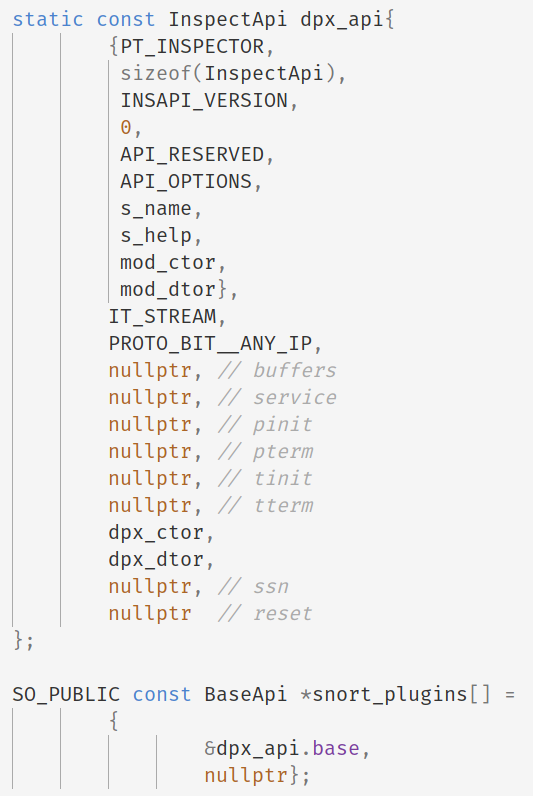
\includegraphics[scale=0.4]{snort1}
    \caption{Đăng ký plugin với snort}
    \label{fig:x cubed graph}
\end{figure}
\FloatBarrier
Khi có gói tin mới đến, snort sẽ gọi đến plugin thông qua hàm eval để xử lý gói tin.
Ở đây ta chỉ chấp nhận các gói tin UDP, TCP và ICMP.
Nếu gói tin bất thường sẽ được gọi đến DetectionEngine của Snort
\begin{figure}[!htbp]
    \centering
    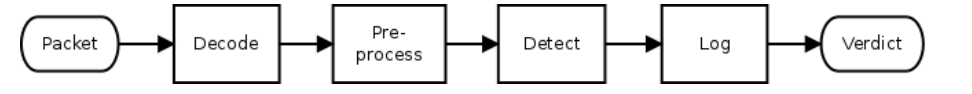
\includegraphics[scale=0.4]{snort2}
    \caption{Hàm xử lý khi có gói tin mới}
    \label{fig:x cubed graph}
\end{figure}
\FloatBarrier
Phân tích gói tin để lấy các thông tin cơ bản riêng biệt chuẩn bị để dự đoán
\begin{figure}[!htbp]
    \centering
    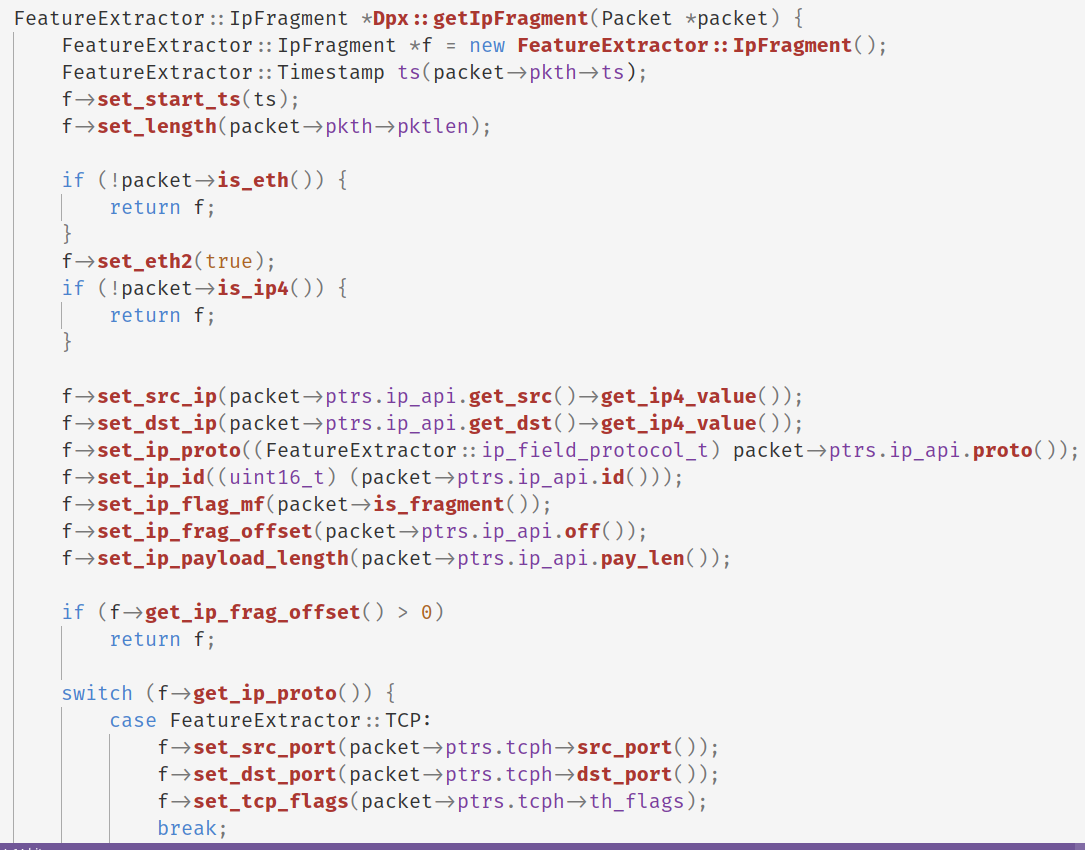
\includegraphics[scale=0.4]{snort6}
    \caption{Phân tích các thông tin cơ bản của gói tin}
    \label{fig:x cubed graph}
\end{figure}
\FloatBarrier
\begin{figure}[!htbp]
    \centering
    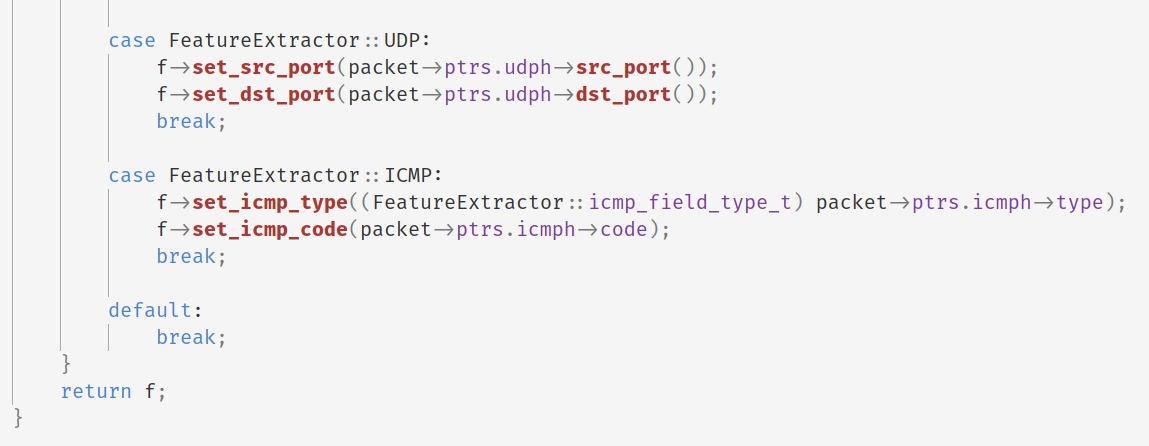
\includegraphics[scale=0.4]{snort7}
    \caption{Phân tích các thông tin cơ bản của gói tin}
    \label{fig:x cubed graph}
\end{figure}
\FloatBarrier
Sau khi trích xuất các thông tin cần thiết từ gói tin, dữ liệu được tách thành 41 features cho dự đoán, 
được mã hóa bằng Flatbuffer
\begin{figure}[!htbp]
    \centering
    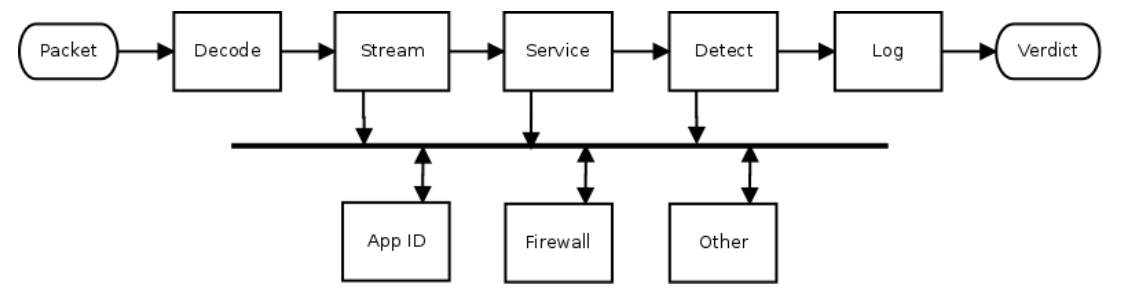
\includegraphics[scale=0.4]{snort3}
    \caption{Mã hóa thông tin gói tin dùng Flatbuffer}
    \label{fig:x cubed graph}
\end{figure}
\FloatBarrier
\begin{figure}[!htbp]
    \centering
    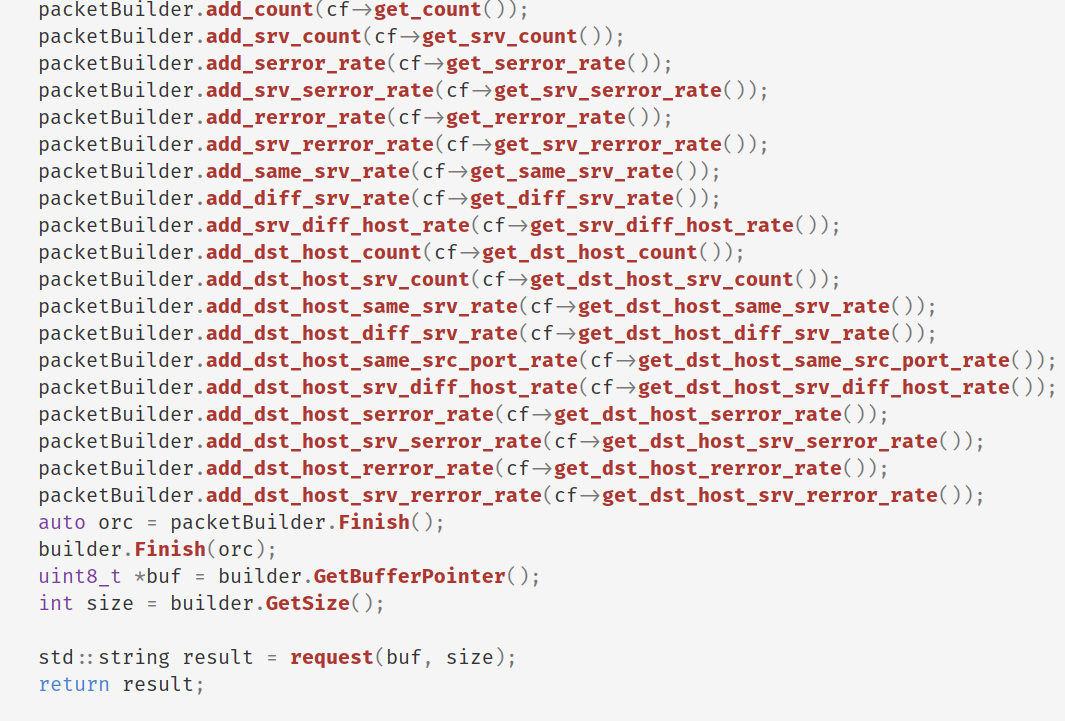
\includegraphics[scale=0.4]{snort4}
    \caption{Mã hóa thông tin gói tin dùng Flatbuffer}
    \label{fig:x cubed graph}
\end{figure}
\FloatBarrier
Sau khi đã phân tích và mã hóa dùng Flatbuffer, chuỗi đã mã hóa được đến máy chủ dự đoán dùng libcurl
\begin{figure}[!htbp]
    \centering
    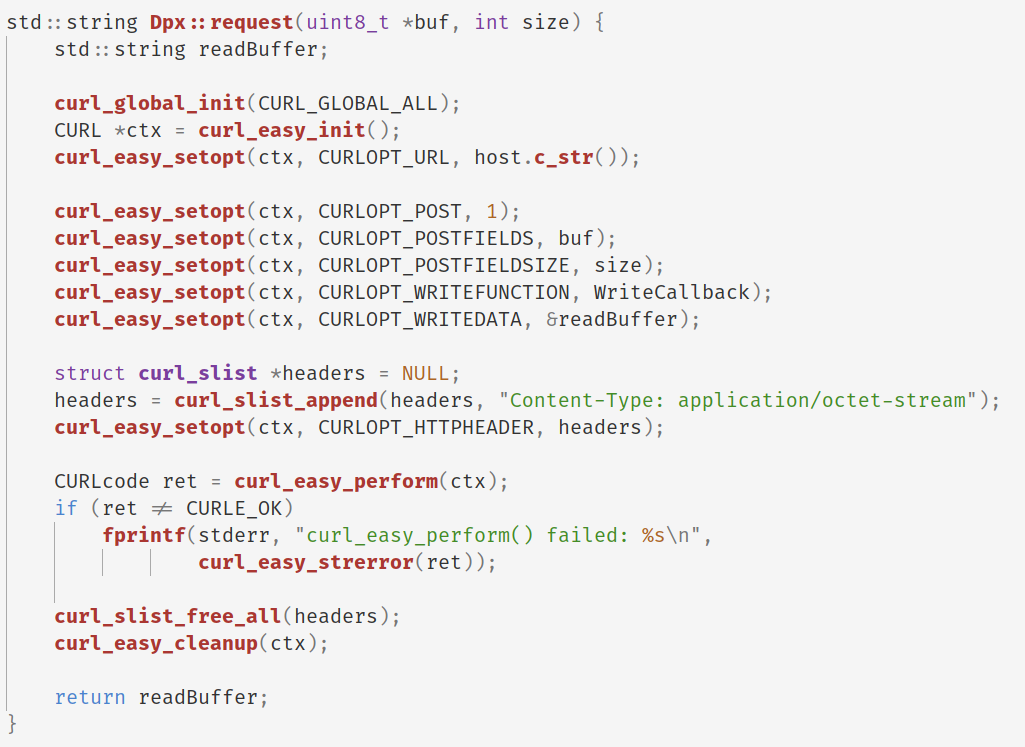
\includegraphics[scale=0.4]{snort5}
    \caption{Gọi đến máy chủ dự đoán}
    \label{fig:x cubed graph}
\end{figure}
\FloatBarrier
\subsection{Máy chủ dự đoán}
Máy chủ dự đoán có nhiệm vụ huấn luyện mạng dự đoán, khởi tạo endpoint /predict để plugin snort gửi yêu cầu http đến kiểm tra gói tin.
Máy chủ cũng cung cấp trang thống kê đơn giản để người dùng quan sát
\begin{figure}[!htbp]
    \centering
    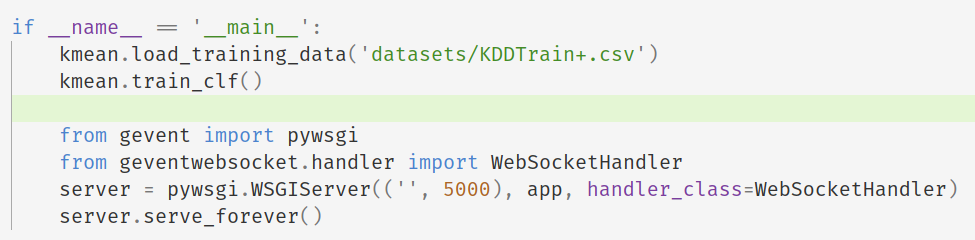
\includegraphics[scale=0.5]{server1}
    \caption{Máy chủ dự đoán}
    \label{fig:x cubed graph}
\end{figure}
\FloatBarrier
\begin{figure}[!htbp]
    \centering
    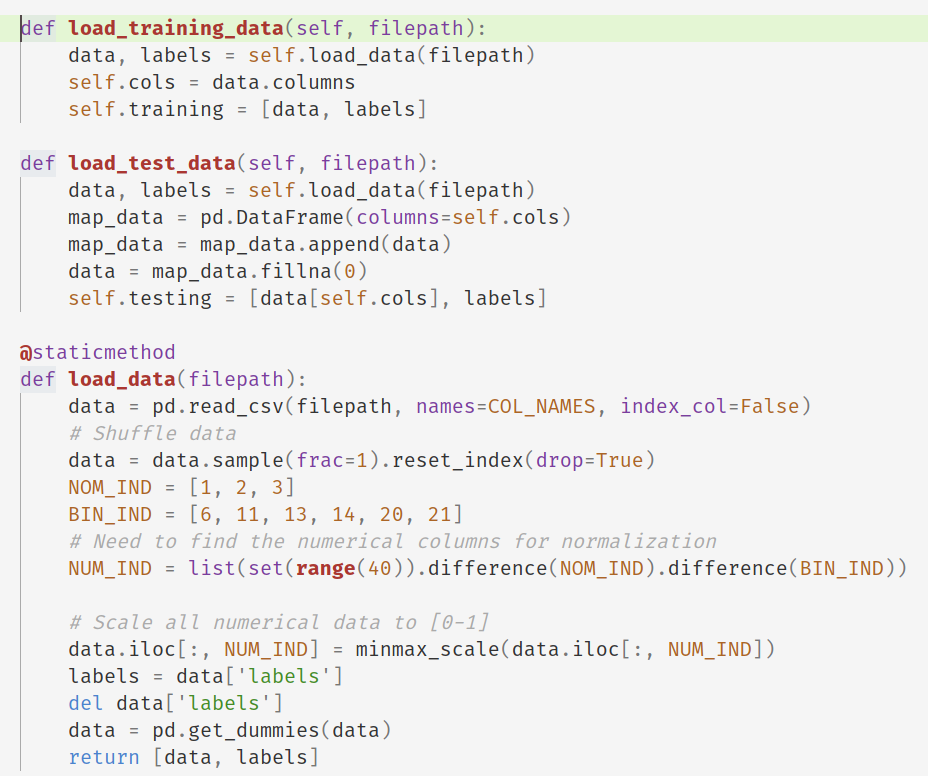
\includegraphics[scale=0.4]{server5}
    \caption{Nhập và xử lý tập dữ liệu}
    \label{fig:x cubed graph}
\end{figure}
\FloatBarrier
\begin{figure}[!htbp]
    \centering
    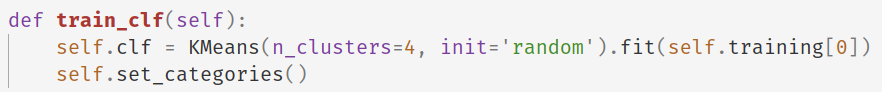
\includegraphics[scale=0.5]{server4}
    \caption{Dùng thuật toán KMeans tạo 4 clusters}
    \label{fig:x cubed graph}
\end{figure}
\FloatBarrier
Endpoint sẽ phân tích request lấy và giải mã Flatbuffer để lấy được cái thông tin gói tin để đưa vào mạng dự đoán
\begin{figure}[!htbp]
    \centering
    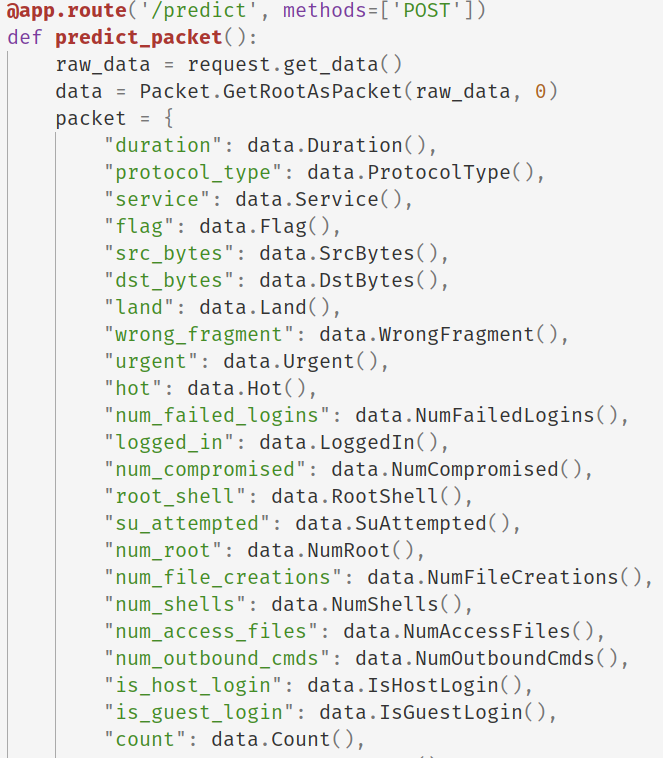
\includegraphics[scale=0.6]{server2}
    \caption{Nhận và giải mã Flatbuffer}
    \label{fig:x cubed graph}
\end{figure}
\FloatBarrier
Sau khi đã giải mã thành công, sẽ đưa vào mạng dự đoán Kmeans để dự đoán và trả về kết quả cho Snort plugin
\begin{figure}[!htbp]
    \centering
    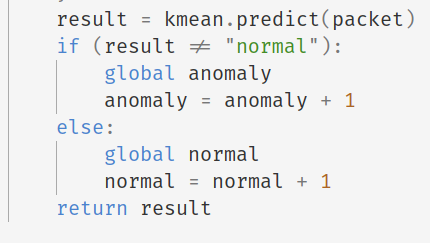
\includegraphics[scale=0.6]{server3}
    \caption{Dự đoán gói tin}
    \label{fig:x cubed graph}
\end{figure}
\FloatBarrier
\section{Thử nghiệm và nhận xét}
\begin{figure}[!htbp]
    \centering
    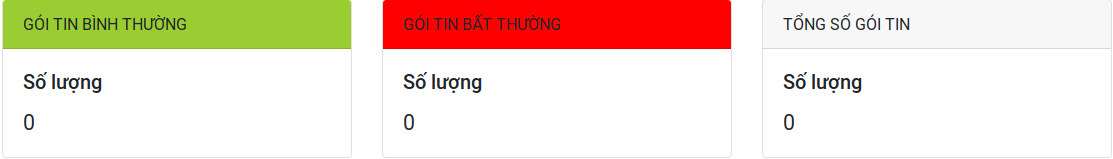
\includegraphics[scale=0.4]{test1}
    \caption{Màn hình thống kê ban đầu}
    \label{fig:x cubed graph}
\end{figure}
\FloatBarrier
\begin{figure}[!htbp]
    \centering
    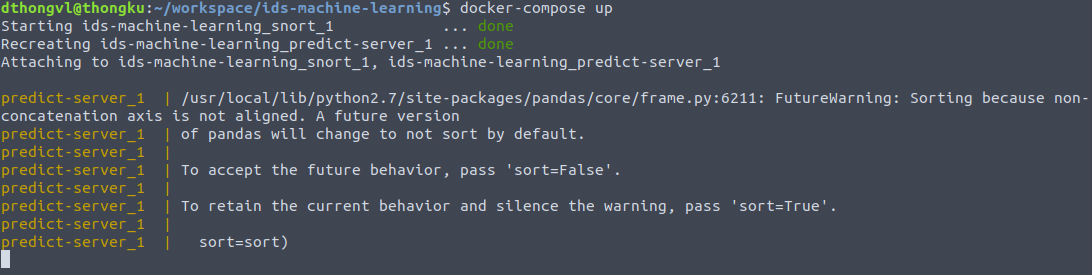
\includegraphics[scale=0.4]{test2}
    \caption{Khởi tạo Docker Compose để thử nghiệm}
    \label{fig:x cubed graph}
\end{figure}
\FloatBarrier
\begin{figure}[!htbp]
    \centering
    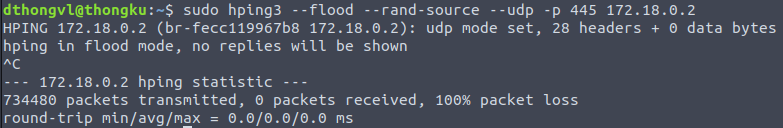
\includegraphics[scale=0.6]{test3}
    \caption{Thử tấn công Ping Flood sử dụng công cụ hping3}
    \label{fig:x cubed graph}
\end{figure}
\FloatBarrier
\begin{figure}[!htbp]
    \centering
    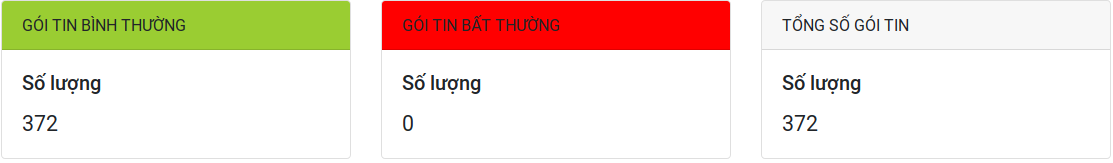
\includegraphics[scale=0.4]{test4}
    \caption{Không phát hiện được tấn công}
    \label{fig:x cubed graph}
\end{figure}
\FloatBarrier
\begin{figure}[!htbp]
    \centering
    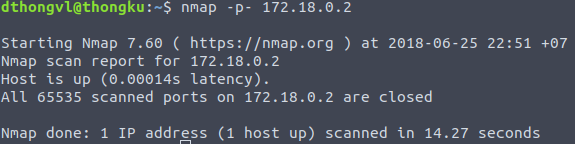
\includegraphics[scale=0.6]{test5}
    \caption{Thử tấn công Scan port bằng công cụ nmap}
    \label{fig:x cubed graph}
\end{figure}
\FloatBarrier
\begin{figure}[!htbp]
    \centering
    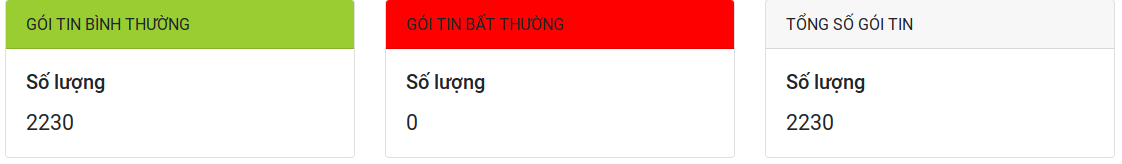
\includegraphics[scale=0.4]{test6}
    \caption{Không phát hiện được tấn công}
    \label{fig:x cubed graph}
\end{figure}
\FloatBarrier